

\tikzset{every picture/.style={line width=0.75pt}} %set default line width to 0.75pt        

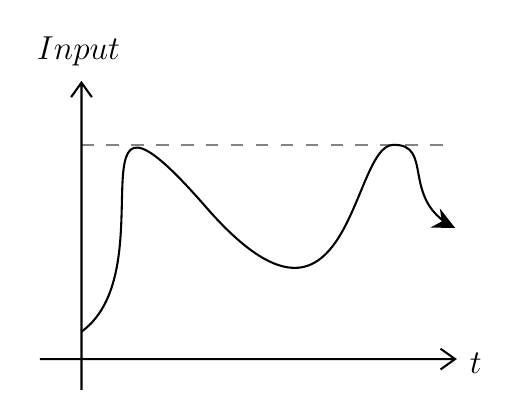
\begin{tikzpicture}[x=0.75pt,y=0.75pt,yscale=-1,xscale=1]
%uncomment if require: \path (0,300); %set diagram left start at 0, and has height of 300

%Straight Lines [id:da26643584263795916] 
\draw [color={rgb, 255:red, 131; green, 131; blue, 131 }  ,draw opacity=1 ] [dash pattern={on 4.5pt off 4.5pt}]  (90,100) -- (270,100) ;


%Shape: Axis 2D [id:dp7046941980103143] 
\draw  (70,203.2) -- (270,203.2)(90,70) -- (90,218) (263,198.2) -- (270,203.2) -- (263,208.2) (85,77) -- (90,70) -- (95,77)  ;
%Curve Lines [id:da03413665677920852] 
\draw    (90,190) .. controls (132.33,159.33) and (80.33,50) .. (150,130) .. controls (219.67,210) and (219.67,100.67) .. (240,100) .. controls (259.93,99.35) and (243.68,125.58) .. (268.43,139.18) ;
\draw [shift={(270,140)}, rotate = 206.28] [fill={rgb, 255:red, 0; green, 0; blue, 0 }  ][line width=0.75]  [draw opacity=0] (10.72,-5.15) -- (0,0) -- (10.72,5.15) -- (7.12,0) -- cycle    ;


% Text Node
\draw (88.5,55) node   {\large $Input$};
% Text Node
\draw (280,205) node   {\large $t$};


\end{tikzpicture}
